\section{Additional Recommendations}\label{sec:additional}

{\bf A small change to the southern portion of the footprint improves overlap with the Euclid footprint} (see \autoref{fig:euclid-overlap}) and causes negligible changes in science metrics. 
\begin{figure}
\centering
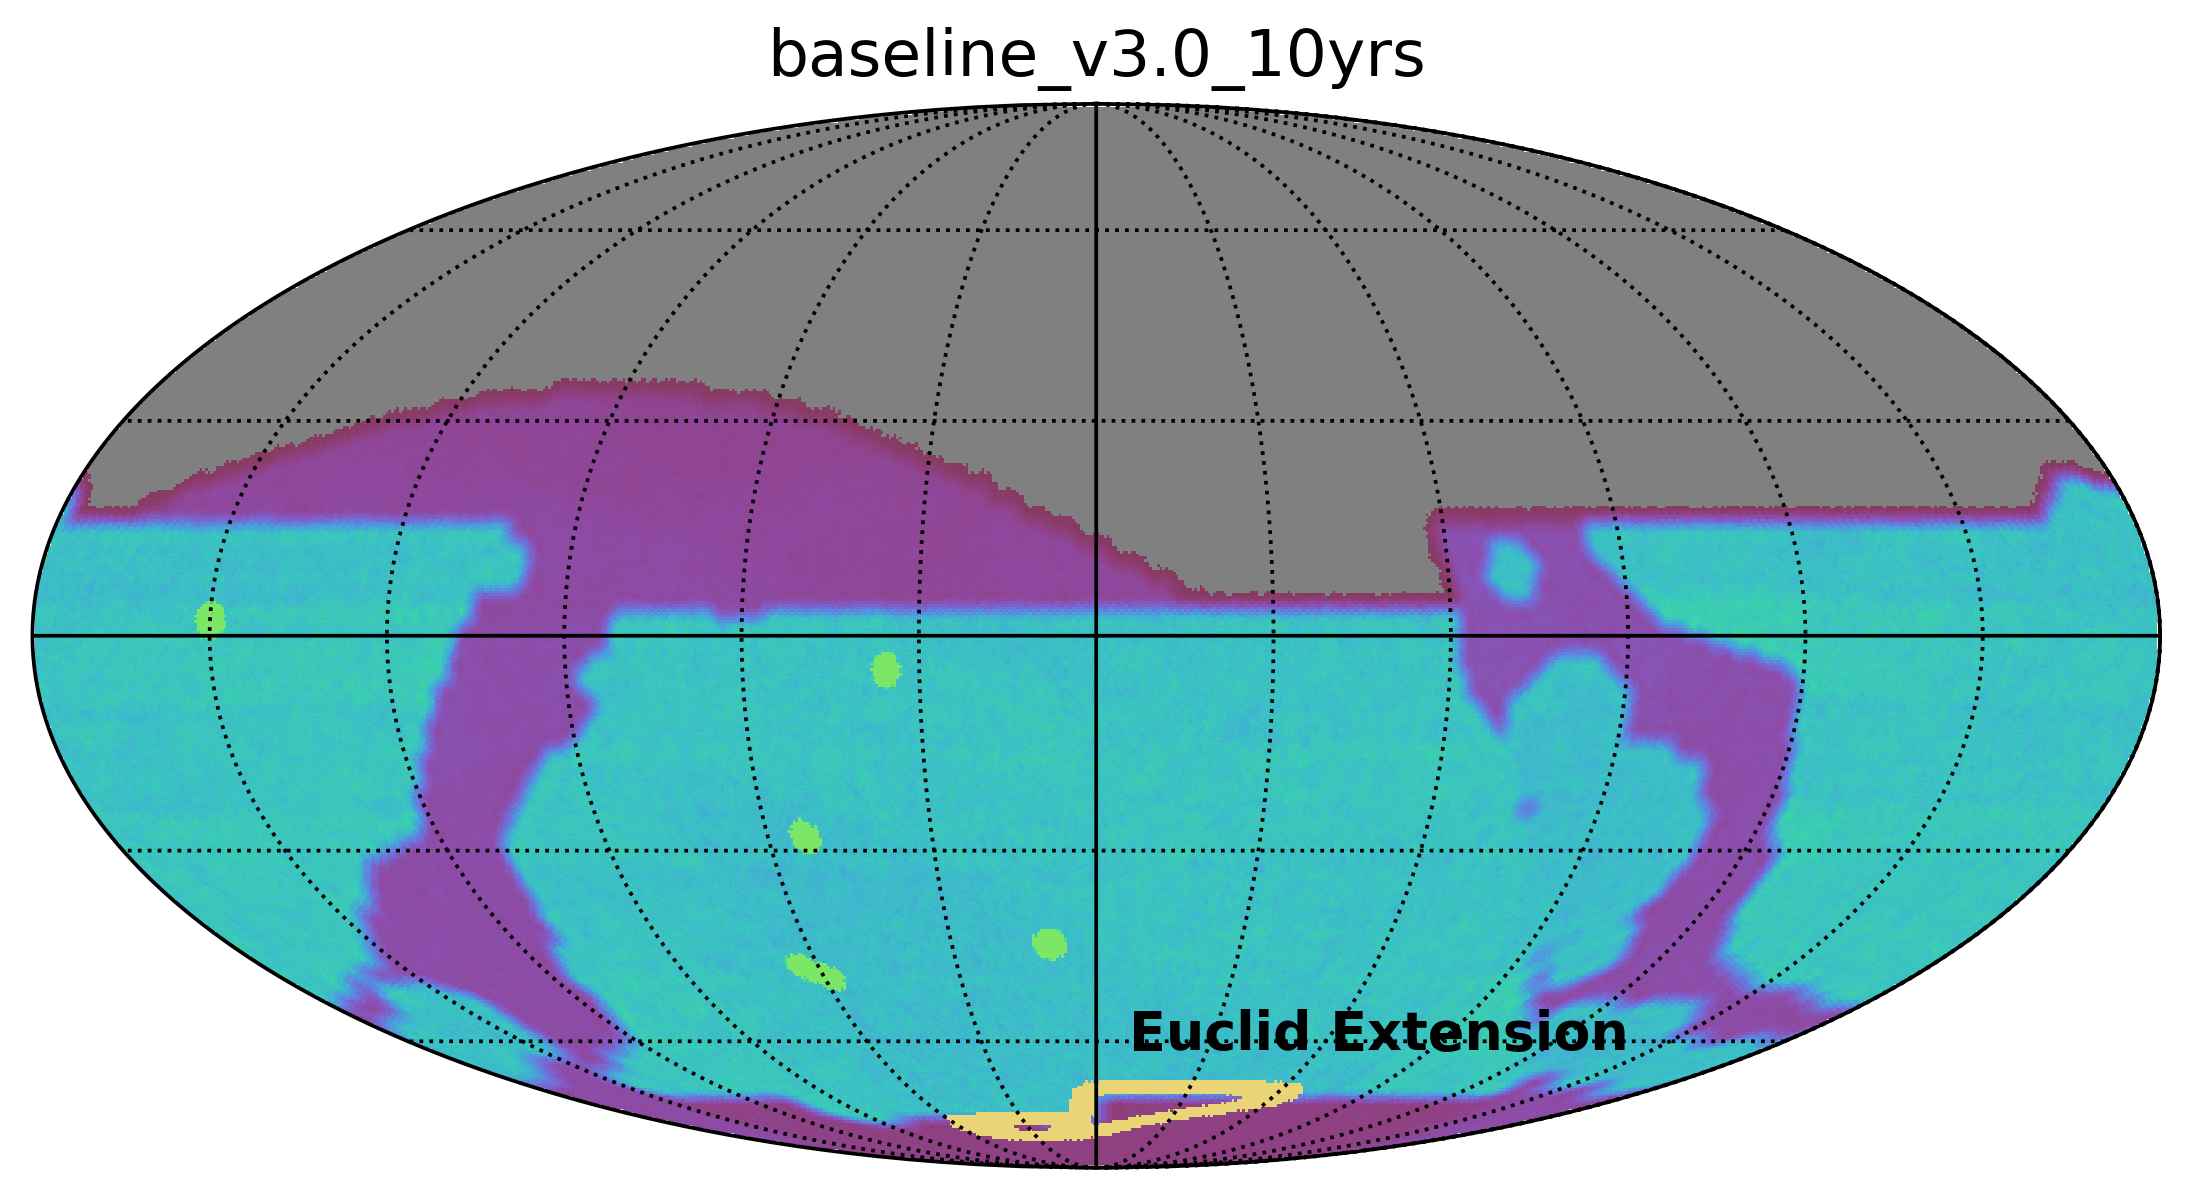
\includegraphics[width=0.45\textwidth]{figures/baseline_v3_0_10yrs_euclid_overlap.png}
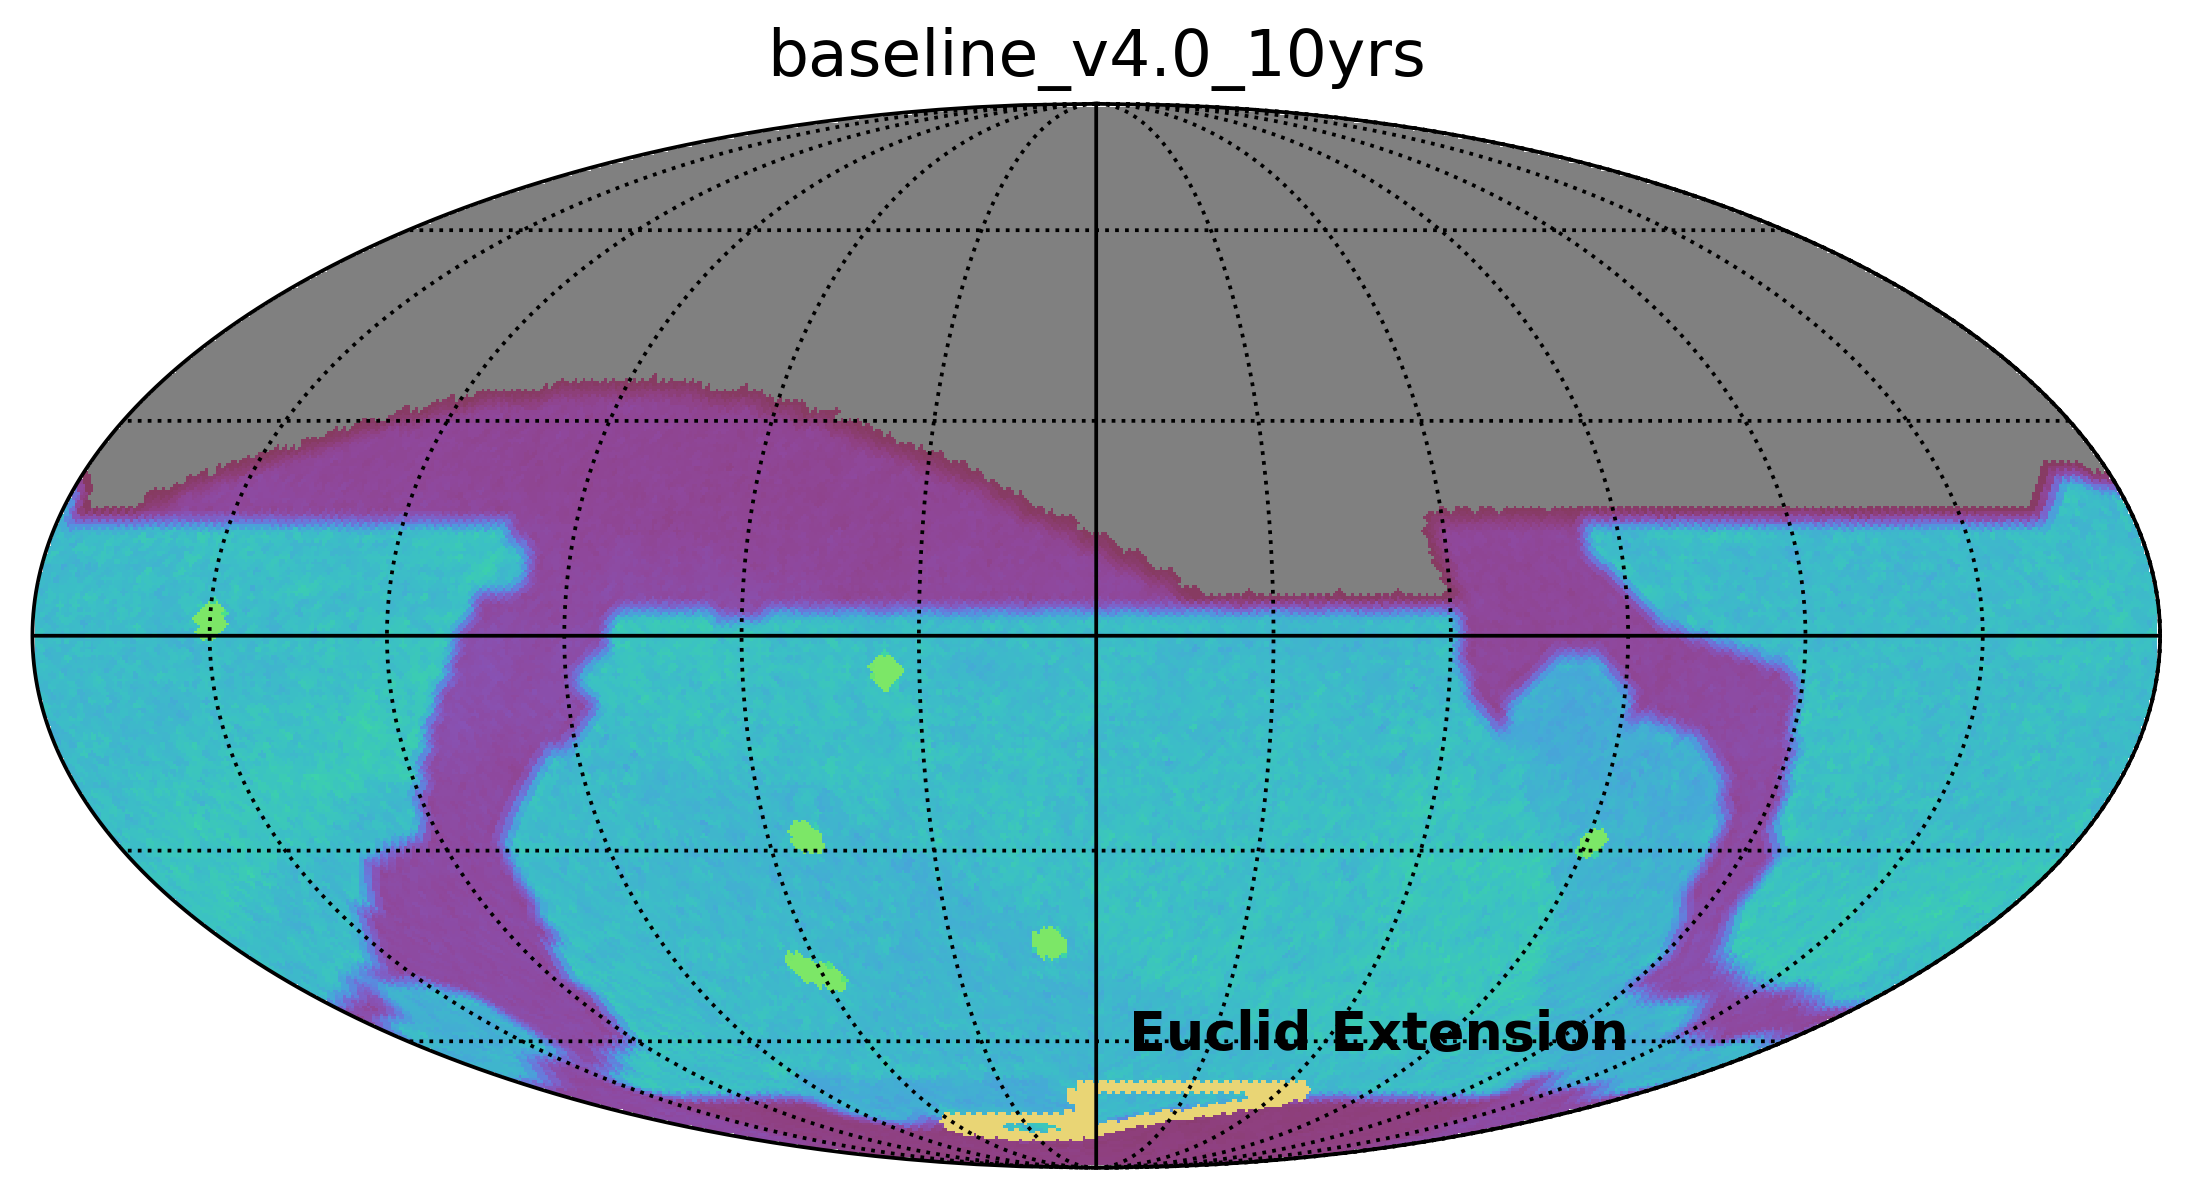
\includegraphics[width=0.45\textwidth]{figures/baseline_v4_0_10yrs_euclid_overlap.png}
%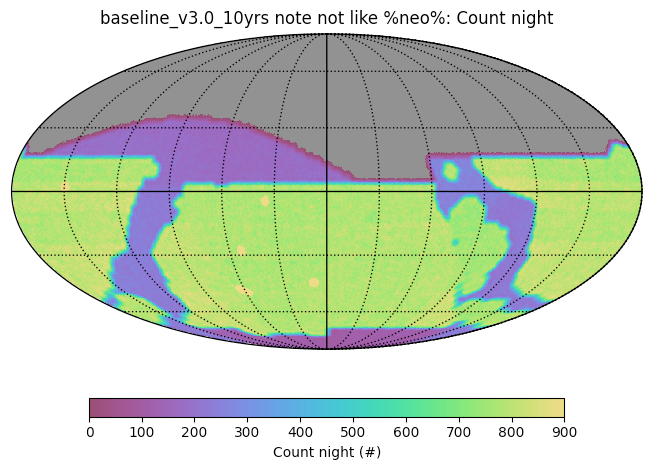
\includegraphics[width=0.45\textwidth]{figures/3.0_south.png}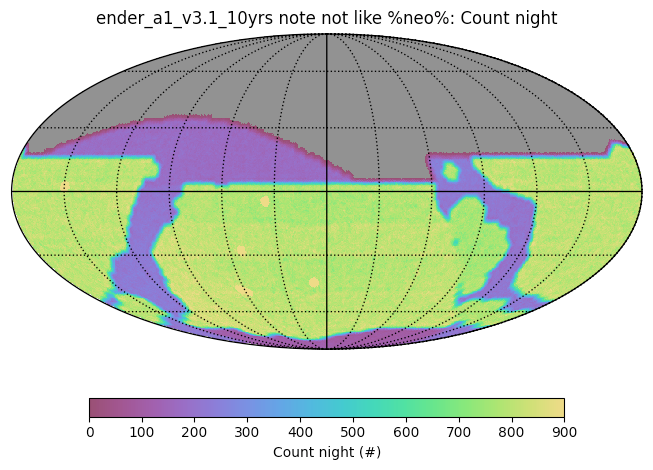
\includegraphics[width=0.45\textwidth]{figures/3.1_south.png}

\caption{Small changes to the southern portion of the footprint improve the overlap with Euclid. \label{fig:euclid-overlap}}
\end{figure}

{\bf The airmass limits for the Near-Sun Twilight microsurvey, introduced with \baseline{3.0}, were increased from $X=2.5$ to $X=3.0$} in \texttt{v3.2}, corresponding to decreasing the minimum solar elongation reached for this microsurvey from 40 degrees to 35 degrees (the range of solar elongations changed from 40 to 60 degrees in \texttt{v3.0} to 35 to 47 degrees in \texttt{v4.0}). This improves the likelihood of discovery of objects with interior-to-Earth orbits, increasing the survey sensitivity to this niche of discovery space. The recovered population of objects
interior to Venus at magnitude $H\leq20$ goes from \mbox{$\sim$4\%} to \mbox{$\sim$40\%} in \texttt{v3.2} and later. The impacts outside the microsurvey are negligible.

\clearpage

\section{Additional changes introduced throughout the \texttt{v3.x} \opsim s } \label{sec:opsimchanges}

Some important assumptions underlying the simulations were updated in Phase 3 of the survey strategy recommendation process: 

\begin{itemize}
\item As of \baseline{3.6}, the downtime in Y1 was increased to reflect a more realistic transition into operations. This change adds approximately eight weeks of downtime reducing the number of visits by \mbox{$\sim$5\%}. The downtime in Y1 is simulated to be maximal early on and decreased to the level expected for the general LSST survey by the end of the first year (\autoref{fig:downtime}). Future simulations will aim to improve the unscheduled downtime model to better align with expectations from the Rubin Observatory Operations team. 

\item As of \baseline{3.6}, the effect of jerk on slew time is included in the simulations, and thus included in scheduling choices. Functionally, this slightly increases the overhead and decreases survey efficiency (\autoref{fig:downtime}).

\begin{figure}[!h]
    \centering
    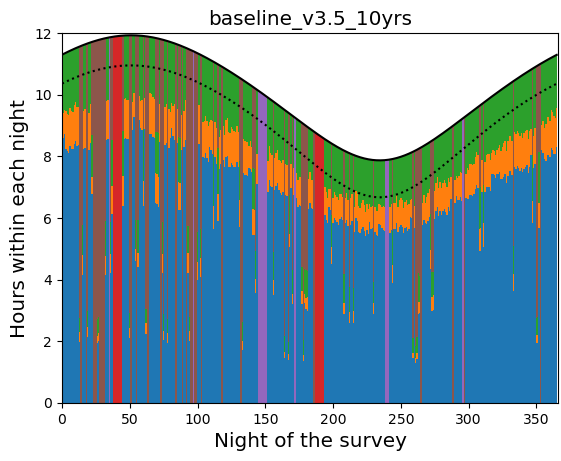
\includegraphics[width=0.37\linewidth]{figures/downtime_v3_5_year1.png}
    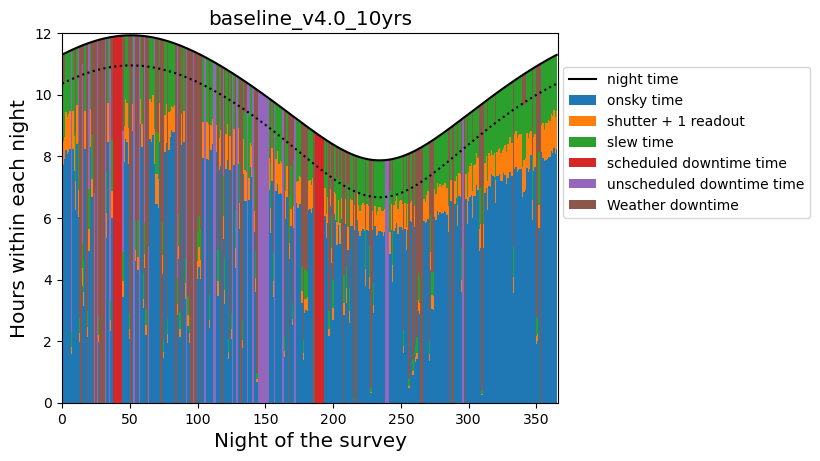
\includegraphics[width=0.37\linewidth]{figures/downtime_v4_0_year1.png}
    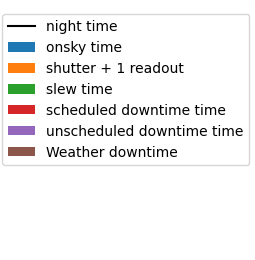
\includegraphics[width=0.24\linewidth]{figures/downtime_v4_0_year1_legend.png}
    \caption{The time within each night of LSST  in Y1 divided into on-sky exposure time, overhead for those exposures (shutter and readout time), time spent slewing, and downtime due to weather, scheduled maintenance activities, or unscheduled engineering. Observing is limited to hours darker than nautical twilight (when the sun is  \mbox{$\leq-$12$\deg$} from the horizon). Before \baseline{3.6} (left plot), simulations only included steady-state expected engineering downtime, modeled as full-night downtime blocks. The \baseline{4.0} simulation (right plot) includes additional unscheduled downtime time within the first 380 nights of the survey, including breaks as short as an hour, to reflect the need for engineering early in the survey. }
    \label{fig:downtime}
\end{figure}


\item The baseline simulations that accompanied the previous SCOC report (\citetalias{PSTN-055}) had a start time of October 1, 2023. As of \baseline{3.2}, the start date of the survey was updated to  May 1, 2025 to match the Project forecast at that time. %The \baseline{4.0} also has a start date of May 1, 2025. 
Future simulations will be updated to match the LSST forecasts.\footnote{\url{ls.st/dates}}. In \texttt{v3.4} we began investigating the effect of changing the start date of the survey. The timing of the start of the survey has an impact on various transient and variable  metrics; the performance changes observed in \autoref{fig:start_dates} are primarily random in nature and generally reflect stochasticity in the metrics themselves, but may also be a result of the interplay between observable sky, rolling schedule, and seasonal weather patterns. The effects are generally comparable with uncertainty associated with weather, as \autoref{fig:startdates_weather} shows.
\end{itemize}

%\begin{figure}
%    \centering
    %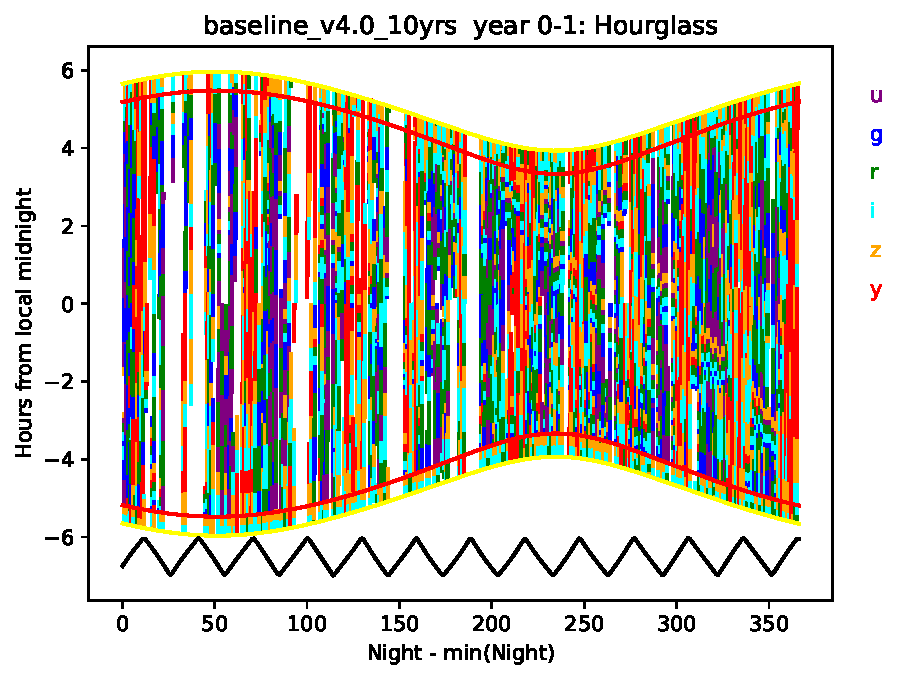
\includegraphics[width=0.75\linewidth]{figures/baseline_v4_0_10yrs_Hourglass_year_0-1_HOUR_Hourglass.pdf}
  %  \caption{This plot shows filter changes per observing night. Downtime (due to weather or telescope scheduled and unscheduled maintenance) is marked by white blocks. Simulations starting with \baseline{3.6} include updated Y1 downtime schedules to reflect realistic expectations of higher downtime periods at the start of the survey. Compared to \baseline{3.5}, \baseline{3.6} and later have approximately eight additional weeks of unscheduled downtime. The impact of the additional downtime is discussed in \autoref{sec:summary}.}
%    \label{fig:enter-label}
%\end{figure}


\begin{figure}
    \centering
    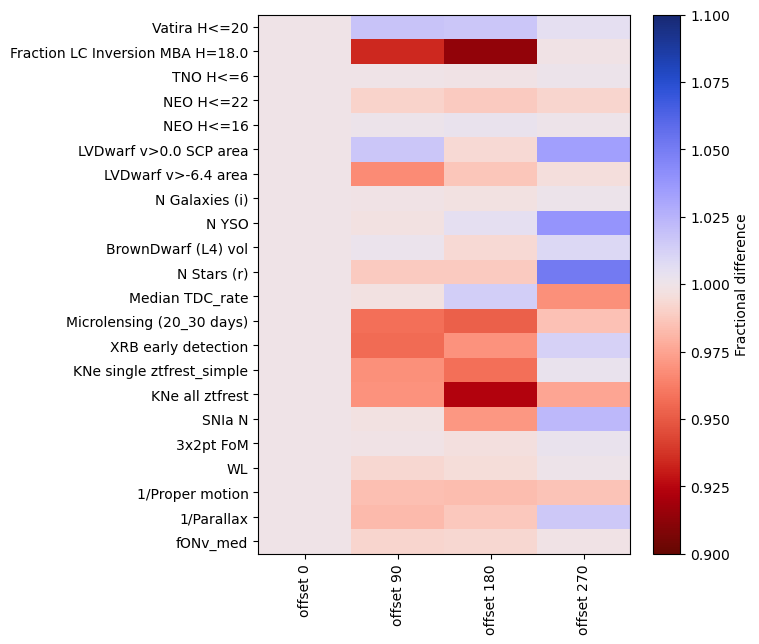
\includegraphics[width=0.9\linewidth]{figures/start_date_scoc_heatmap.png}
    \caption{Performance of a subset of key metrics for implementations of \baseline{3.4} with different start dates, offset by ``offset'' days from the May 1, 2025. Seasonal weather patterns interact with scheduler choices and the timing of rolling. Static science metrics are generally unchanged or only marginally affected, while transient and variable science sees larger impacts. }
    \label{fig:start_dates}
\end{figure}


\begin{figure}
    \centering
    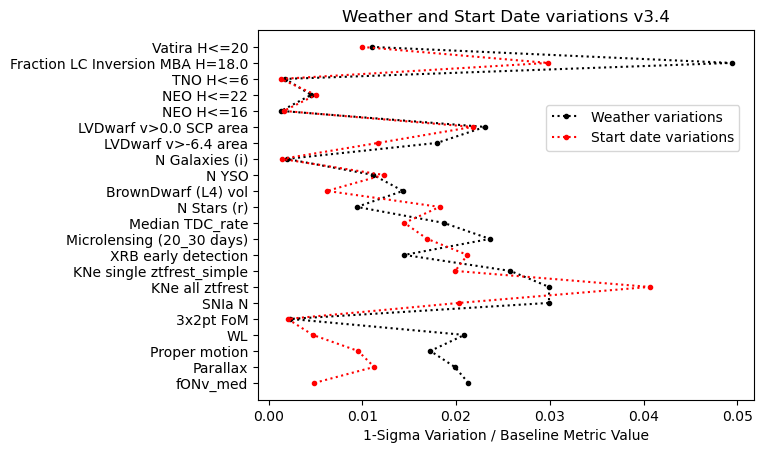
\includegraphics[width=0.85\linewidth]{figures/uncertainties_v3_4.png}
    \caption{In the \texttt{v3.4} \opsim\ family, we ran an extensive set of variations on both the time of year when the survey starts and the cloud history period sampled in the simulations. Both factors produce variations in metric results of similar magnitude. This reflects the effect of the dynamic scheduler's responses to weather and the current state of the survey. The figure shows the level of (1-sigma) uncertainties in metrics due to these events.} %to the uncertainty observed changing the start date of the survey, demonstrating that the effect of start date changes is dominated by weather-related effects.}
    \label{fig:startdates_weather}
\end{figure}
\clearpage